\documentclass[twoside]{book}

% Packages required by doxygen
\usepackage{calc}
\usepackage{doxygen}
\usepackage{graphicx}
\usepackage[utf8]{inputenc}
\usepackage{makeidx}
\usepackage{multicol}
\usepackage{multirow}
\usepackage{fixltx2e}
\PassOptionsToPackage{warn}{textcomp}
\usepackage{textcomp}
\usepackage[nointegrals]{wasysym}
\usepackage[table]{xcolor}

% Font selection
\usepackage[T1]{fontenc}
\usepackage{mathptmx}
\usepackage[scaled=.90]{helvet}
\usepackage{courier}
\usepackage{amssymb}
\usepackage{sectsty}
\renewcommand{\familydefault}{\sfdefault}
\allsectionsfont{%
  \fontseries{bc}\selectfont%
  \color{darkgray}%
}
\renewcommand{\DoxyLabelFont}{%
  \fontseries{bc}\selectfont%
  \color{darkgray}%
}
\newcommand{\+}{\discretionary{\mbox{\scriptsize$\hookleftarrow$}}{}{}}

% Page & text layout
\usepackage{geometry}
\geometry{%
  a4paper,%
  top=2.5cm,%
  bottom=2.5cm,%
  left=2.5cm,%
  right=2.5cm%
}
\tolerance=750
\hfuzz=15pt
\hbadness=750
\setlength{\emergencystretch}{15pt}
\setlength{\parindent}{0cm}
\setlength{\parskip}{0.2cm}
\makeatletter
\renewcommand{\paragraph}{%
  \@startsection{paragraph}{4}{0ex}{-1.0ex}{1.0ex}{%
    \normalfont\normalsize\bfseries\SS@parafont%
  }%
}
\renewcommand{\subparagraph}{%
  \@startsection{subparagraph}{5}{0ex}{-1.0ex}{1.0ex}{%
    \normalfont\normalsize\bfseries\SS@subparafont%
  }%
}
\makeatother

% Headers & footers
\usepackage{fancyhdr}
\pagestyle{fancyplain}
\fancyhead[LE]{\fancyplain{}{\bfseries\thepage}}
\fancyhead[CE]{\fancyplain{}{}}
\fancyhead[RE]{\fancyplain{}{\bfseries\leftmark}}
\fancyhead[LO]{\fancyplain{}{\bfseries\rightmark}}
\fancyhead[CO]{\fancyplain{}{}}
\fancyhead[RO]{\fancyplain{}{\bfseries\thepage}}
\fancyfoot[LE]{\fancyplain{}{}}
\fancyfoot[CE]{\fancyplain{}{}}
\fancyfoot[RE]{\fancyplain{}{\bfseries\scriptsize Generated on Thu May 29 2014 22\+:58\+:14 for My Project by Doxygen }}
\fancyfoot[LO]{\fancyplain{}{\bfseries\scriptsize Generated on Thu May 29 2014 22\+:58\+:14 for My Project by Doxygen }}
\fancyfoot[CO]{\fancyplain{}{}}
\fancyfoot[RO]{\fancyplain{}{}}
\renewcommand{\footrulewidth}{0.4pt}
\renewcommand{\chaptermark}[1]{%
  \markboth{#1}{}%
}
\renewcommand{\sectionmark}[1]{%
  \markright{\thesection\ #1}%
}

% Indices & bibliography
\usepackage{natbib}
\usepackage[titles]{tocloft}
\setcounter{tocdepth}{3}
\setcounter{secnumdepth}{5}
\makeindex

% Hyperlinks (required, but should be loaded last)
\usepackage{ifpdf}
\ifpdf
  \usepackage[pdftex,pagebackref=true]{hyperref}
\else
  \usepackage[ps2pdf,pagebackref=true]{hyperref}
\fi
\hypersetup{%
  colorlinks=true,%
  linkcolor=blue,%
  citecolor=blue,%
  unicode%
}

% Custom commands
\newcommand{\clearemptydoublepage}{%
  \newpage{\pagestyle{empty}\cleardoublepage}%
}


%===== C O N T E N T S =====

\begin{document}

% Titlepage & ToC
\hypersetup{pageanchor=false,
             bookmarks=true,
             bookmarksnumbered=true,
             pdfencoding=unicode
            }
\pagenumbering{roman}
\begin{titlepage}
\vspace*{7cm}
\begin{center}%
{\Large My Project }\\
\vspace*{1cm}
{\large Generated by Doxygen 1.8.7}\\
\vspace*{0.5cm}
{\small Thu May 29 2014 22:58:14}\\
\end{center}
\end{titlepage}
\clearemptydoublepage
\tableofcontents
\clearemptydoublepage
\pagenumbering{arabic}
\hypersetup{pageanchor=true}

%--- Begin generated contents ---
\chapter{Hierarchical Index}
\section{Class Hierarchy}
This inheritance list is sorted roughly, but not completely, alphabetically\+:\begin{DoxyCompactList}
\item \contentsline{section}{Config}{\pageref{struct_config}}{}
\item \contentsline{section}{Configuration}{\pageref{struct_configuration}}{}
\item \contentsline{section}{Conv\+Net}{\pageref{class_conv_net}}{}
\item \contentsline{section}{Layer}{\pageref{class_layer}}{}
\begin{DoxyCompactList}
\item \contentsline{section}{Conv\+Layer}{\pageref{class_conv_layer}}{}
\item \contentsline{section}{Fully\+Connected\+Layer}{\pageref{class_fully_connected_layer}}{}
\end{DoxyCompactList}
\end{DoxyCompactList}

\chapter{Class Index}
\section{Class List}
Here are the classes, structs, unions and interfaces with brief descriptions\+:\begin{DoxyCompactList}
\item\contentsline{section}{\hyperlink{class_conv_layer}{Conv\+Layer} }{\pageref{class_conv_layer}}{}
\end{DoxyCompactList}

\chapter{File Index}
\section{File List}
Here is a list of all documented files with brief descriptions\+:\begin{DoxyCompactList}
\item\contentsline{section}{/\+Users/chengtai/\+Documents/2014/\+M\+O\+T\+R/modules/\+Alpha/\+Alpha/{\bfseries configuration.\+h} }{\pageref{configuration_8h}}{}
\item\contentsline{section}{/\+Users/chengtai/\+Documents/2014/\+M\+O\+T\+R/modules/\+Alpha/\+Alpha/{\bfseries convnet.\+h} }{\pageref{convnet_8h}}{}
\item\contentsline{section}{/\+Users/chengtai/\+Documents/2014/\+M\+O\+T\+R/modules/\+Alpha/\+Alpha/{\bfseries helper.\+h} }{\pageref{helper_8h}}{}
\item\contentsline{section}{/\+Users/chengtai/\+Documents/2014/\+M\+O\+T\+R/modules/\+Alpha/\+Alpha/\hyperlink{layer_8h}{layer.\+h} }{\pageref{layer_8h}}{}
\item\contentsline{section}{/\+Users/chengtai/\+Documents/2014/\+M\+O\+T\+R/modules/\+Alpha/\+Alpha/{\bfseries test.\+h} }{\pageref{test_8h}}{}
\item\contentsline{section}{/\+Users/chengtai/\+Documents/2014/\+M\+O\+T\+R/modules/\+Alpha/\+Alpha/{\bfseries utils.\+h} }{\pageref{utils_8h}}{}
\item\contentsline{section}{/\+Users/chengtai/\+Documents/2014/\+M\+O\+T\+R/modules/\+Alpha/\+Alpha/{\bfseries visual.\+h} }{\pageref{visual_8h}}{}
\end{DoxyCompactList}

\chapter{Class Documentation}
\hypertarget{struct_config}{\section{Config Struct Reference}
\label{struct_config}\index{Config@{Config}}
}
\subsection*{Public Attributes}
\begin{DoxyCompactItemize}
\item 
\hypertarget{struct_config_a8482c2a80bd7661adefb7e4af2c8e82f}{int \hyperlink{struct_config_a8482c2a80bd7661adefb7e4af2c8e82f}{ninmaps}}\label{struct_config_a8482c2a80bd7661adefb7e4af2c8e82f}

\begin{DoxyCompactList}\small\item\em for convlayers. \end{DoxyCompactList}\item 
\hypertarget{struct_config_ab7f363b2ca498b13f6e1fe9cb3772c16}{int {\bfseries inputrows}}\label{struct_config_ab7f363b2ca498b13f6e1fe9cb3772c16}

\item 
\hypertarget{struct_config_a236752a83d954c43bd21a0731173eec0}{int {\bfseries inputcols}}\label{struct_config_a236752a83d954c43bd21a0731173eec0}

\item 
\hypertarget{struct_config_ad7a985e951722129907736ae5c092459}{int {\bfseries stride}}\label{struct_config_ad7a985e951722129907736ae5c092459}

\item 
\hypertarget{struct_config_aef9875c26e3c553b843359901a6083a6}{int {\bfseries side}}\label{struct_config_aef9875c26e3c553b843359901a6083a6}

\item 
\hypertarget{struct_config_a39ebc108302ce9a999b45cb6dfb3d386}{int {\bfseries kernelsize}}\label{struct_config_a39ebc108302ce9a999b45cb6dfb3d386}

\item 
\hypertarget{struct_config_ad85769049d1ef3cdca4b31486aa2128e}{int {\bfseries noutmaps}}\label{struct_config_ad85769049d1ef3cdca4b31486aa2128e}

\item 
\hypertarget{struct_config_ae694bea0336597df1a264b6352440abb}{bool {\bfseries isdownsample}}\label{struct_config_ae694bea0336597df1a264b6352440abb}

\item 
\hypertarget{struct_config_a095d32cd326378d067389be47e85ea82}{vector$<$ set$<$ int $>$ $>$ {\bfseries inmaps}}\label{struct_config_a095d32cd326378d067389be47e85ea82}

\item 
\hypertarget{struct_config_afb439e83ef17afef86cc30f5caa2f433}{int \hyperlink{struct_config_afb439e83ef17afef86cc30f5caa2f433}{fanin}}\label{struct_config_afb439e83ef17afef86cc30f5caa2f433}

\begin{DoxyCompactList}\small\item\em for fully connected layers. \end{DoxyCompactList}\item 
\hypertarget{struct_config_a53c21449d6147fbd7023f158e109cb4d}{int {\bfseries fanout}}\label{struct_config_a53c21449d6147fbd7023f158e109cb4d}

\end{DoxyCompactItemize}


The documentation for this struct was generated from the following file\+:\begin{DoxyCompactItemize}
\item 
/\+Users/chengtai/\+Documents/2014/\+M\+O\+T\+R/modules/\+Alpha/\+Alpha/configuration.\+h\end{DoxyCompactItemize}

\hypertarget{struct_configuration}{\section{Configuration Struct Reference}
\label{struct_configuration}\index{Configuration@{Configuration}}
}
\subsection*{Public Attributes}
\begin{DoxyCompactItemize}
\item 
\hypertarget{struct_configuration_a0a011834331cc1da7029d8b11f8234c8}{int {\bfseries nconvlayers}}\label{struct_configuration_a0a011834331cc1da7029d8b11f8234c8}

\item 
\hypertarget{struct_configuration_ad1f3df350b8795f714c10ef2c641bdb9}{int {\bfseries nfclayers}}\label{struct_configuration_ad1f3df350b8795f714c10ef2c641bdb9}

\item 
\hypertarget{struct_configuration_ae770a2fe69b45d01bb20597ee8f6898b}{vector$<$ \hyperlink{struct_config}{Config} $>$ {\bfseries vconfig}}\label{struct_configuration_ae770a2fe69b45d01bb20597ee8f6898b}

\end{DoxyCompactItemize}


The documentation for this struct was generated from the following file\+:\begin{DoxyCompactItemize}
\item 
/\+Users/chengtai/\+Documents/2014/\+M\+O\+T\+R/modules/\+Alpha/\+Alpha/configuration.\+h\end{DoxyCompactItemize}

\hypertarget{class_conv_layer}{\section{Conv\+Layer Class Reference}
\label{class_conv_layer}\index{Conv\+Layer@{Conv\+Layer}}
}
Inheritance diagram for Conv\+Layer\+:\begin{figure}[H]
\begin{center}
\leavevmode
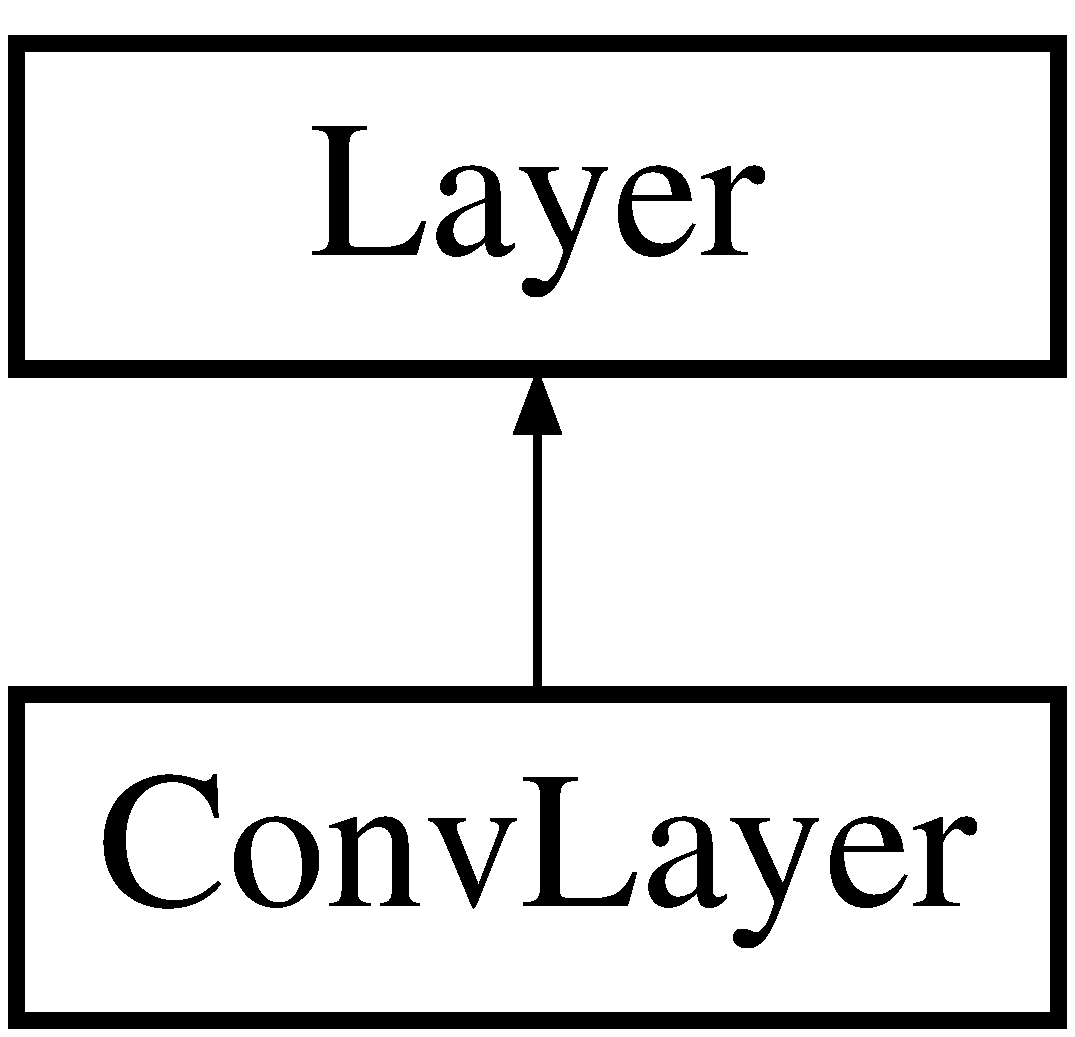
\includegraphics[height=2.000000cm]{class_conv_layer}
\end{center}
\end{figure}
\subsection*{Public Member Functions}
\begin{DoxyCompactItemize}
\item 
\hyperlink{class_conv_layer_a7516441d146b575d8ba191278fe8ba9d}{Conv\+Layer} (int \+\_\+ninmaps, int \+\_\+inputrows, int \+\_\+inputcols, int \+\_\+noutmaps, int \+\_\+stride, int \+\_\+side, int \+\_\+kernelsize, vector$<$ Mat\+Type $>$ $\ast$\+\_\+indata=N\+U\+L\+L)
\item 
\hypertarget{class_conv_layer_ad7b04710a903116d88fcc017b2ca4f2f}{void {\bfseries Set\+Filter} (const vector$<$ vector$<$ Filter\+Type $>$ $>$ \&)}\label{class_conv_layer_ad7b04710a903116d88fcc017b2ca4f2f}

\item 
\hypertarget{class_conv_layer_a585102c25508332b6ab2799409393204}{void {\bfseries Set\+Input} (vector$<$ Mat\+Type $>$ $\ast$)}\label{class_conv_layer_a585102c25508332b6ab2799409393204}

\item 
\hypertarget{class_conv_layer_a8bb67f36834497242e12d0eea4ece95a}{void {\bfseries Set\+Inmaps} (const vector$<$ set$<$ int $>$ $>$ \&)}\label{class_conv_layer_a8bb67f36834497242e12d0eea4ece95a}

\item 
\hypertarget{class_conv_layer_a70111098046a07416fcbdffdbe8f0cfd}{void \hyperlink{class_conv_layer_a70111098046a07416fcbdffdbe8f0cfd}{Apply\+Filter} ()}\label{class_conv_layer_a70111098046a07416fcbdffdbe8f0cfd}

\begin{DoxyCompactList}\small\item\em T\+O\+D\+O\+: the index order is filter\mbox{[}j\mbox{]}\mbox{[}i\mbox{]}, inmaps\mbox{[}j\mbox{]}\mbox{[}i\mbox{]}, not the other way around. \end{DoxyCompactList}\item 
\hypertarget{class_conv_layer_a8970249425ba935d91bc0f0a530ea13c}{void {\bfseries Down\+Sample} ()}\label{class_conv_layer_a8970249425ba935d91bc0f0a530ea13c}

\item 
\hypertarget{class_conv_layer_a5e5a5da58cb21ca2894ecf55088a2636}{void {\bfseries Apply\+Nonlinearity} ()}\label{class_conv_layer_a5e5a5da58cb21ca2894ecf55088a2636}

\item 
\hypertarget{class_conv_layer_aea08727ba47d3c813e309cc278860bbd}{bool {\bfseries Self\+Check} ()}\label{class_conv_layer_aea08727ba47d3c813e309cc278860bbd}

\end{DoxyCompactItemize}
\subsection*{Public Attributes}
\begin{DoxyCompactItemize}
\item 
\hypertarget{class_conv_layer_a3fbf8929ebf39d70281c548653159fe1}{vector$<$ vector$<$ Filter\+Type $>$ $>$ {\bfseries filter}}\label{class_conv_layer_a3fbf8929ebf39d70281c548653159fe1}

\item 
\hypertarget{class_conv_layer_ae90ccdaf98509ac518dc8158abb53540}{vector$<$ Mat\+Type $>$ $\ast$ {\bfseries indata}}\label{class_conv_layer_ae90ccdaf98509ac518dc8158abb53540}

\item 
\hypertarget{class_conv_layer_a41e52948623d345d93ddf7e3e6d4098c}{vector$<$ Mat\+Type $>$ {\bfseries outdata}}\label{class_conv_layer_a41e52948623d345d93ddf7e3e6d4098c}

\item 
\hypertarget{class_conv_layer_a2a829e399b291ef09856b71484ddcade}{vector$<$ set$<$ int $>$ $>$ {\bfseries inmaps}}\label{class_conv_layer_a2a829e399b291ef09856b71484ddcade}

\item 
\hypertarget{class_conv_layer_a9c41797df74c1eef60fb4fdbf2713379}{string {\bfseries name}}\label{class_conv_layer_a9c41797df74c1eef60fb4fdbf2713379}

\item 
\hypertarget{class_conv_layer_a62ef7802fa2cb90f2a6c3f09f52d1485}{const int {\bfseries ninmaps}}\label{class_conv_layer_a62ef7802fa2cb90f2a6c3f09f52d1485}

\item 
\hypertarget{class_conv_layer_a24e3feabcb086d6a9985c263b954f32e}{const int {\bfseries inputrows}}\label{class_conv_layer_a24e3feabcb086d6a9985c263b954f32e}

\item 
\hypertarget{class_conv_layer_a51c24316490e75baea4950781a65d7f9}{const int {\bfseries inputcols}}\label{class_conv_layer_a51c24316490e75baea4950781a65d7f9}

\item 
\hypertarget{class_conv_layer_a5b16865e198761926c2f4820062b0766}{const int {\bfseries noutmaps}}\label{class_conv_layer_a5b16865e198761926c2f4820062b0766}

\item 
\hypertarget{class_conv_layer_a503460202a6877759475b94e8bda8aa6}{const int {\bfseries stride}}\label{class_conv_layer_a503460202a6877759475b94e8bda8aa6}

\item 
\hypertarget{class_conv_layer_aa393a1694d13a8d62f3eddc1709e5b74}{const int {\bfseries side}}\label{class_conv_layer_aa393a1694d13a8d62f3eddc1709e5b74}

\item 
\hypertarget{class_conv_layer_ad0f8a1eab56d2db1309913de2b299fc9}{const int {\bfseries kernelsize}}\label{class_conv_layer_ad0f8a1eab56d2db1309913de2b299fc9}

\end{DoxyCompactItemize}


\subsection{Constructor \& Destructor Documentation}
\hypertarget{class_conv_layer_a7516441d146b575d8ba191278fe8ba9d}{\index{Conv\+Layer@{Conv\+Layer}!Conv\+Layer@{Conv\+Layer}}
\index{Conv\+Layer@{Conv\+Layer}!Conv\+Layer@{Conv\+Layer}}
\subsubsection[{Conv\+Layer}]{\setlength{\rightskip}{0pt plus 5cm}Conv\+Layer\+::\+Conv\+Layer (
\begin{DoxyParamCaption}
\item[{int}]{\+\_\+ninmaps, }
\item[{int}]{\+\_\+inputrows, }
\item[{int}]{\+\_\+inputcols, }
\item[{int}]{\+\_\+noutmaps, }
\item[{int}]{\+\_\+stride, }
\item[{int}]{\+\_\+side, }
\item[{int}]{\+\_\+kernelsize, }
\item[{vector$<$ Mat\+Type $>$ $\ast$}]{\+\_\+indata = {\ttfamily NULL}}
\end{DoxyParamCaption}
)\hspace{0.3cm}{\ttfamily [inline]}}}\label{class_conv_layer_a7516441d146b575d8ba191278fe8ba9d}

\begin{DoxyParams}{Parameters}
{\em \+\_\+ninmaps} & Number of input maps. \\
\hline
{\em \+\_\+inputrows} & Number of rows of input matrix. \\
\hline
{\em \+\_\+inputcols} & Number of columns of input matrix. \\
\hline
{\em \+\_\+noutmaps} & Number of maps of this layer. \\
\hline
{\em \+\_\+stride} & stride. \\
\hline
{\em \+\_\+side} & side. \\
\hline
{\em \+\_\+kernelsize} & kernelsize, must be square. \\
\hline
{\em \+\_\+indata.} & Input data, optional. \\
\hline
\end{DoxyParams}


The documentation for this class was generated from the following files\+:\begin{DoxyCompactItemize}
\item 
/\+Users/chengtai/\+Documents/2014/\+M\+O\+T\+R/modules/\+Alpha/\+Alpha/\hyperlink{layer_8h}{layer.\+h}\item 
/\+Users/chengtai/\+Documents/2014/\+M\+O\+T\+R/modules/\+Alpha/\+Alpha/layer.\+cpp\end{DoxyCompactItemize}

\hypertarget{class_conv_net}{\section{Conv\+Net Class Reference}
\label{class_conv_net}\index{Conv\+Net@{Conv\+Net}}
}
\subsection*{Public Member Functions}
\begin{DoxyCompactItemize}
\item 
\hypertarget{class_conv_net_a1494deafc867bf0a25ff4adb748cb9d5}{void {\bfseries Setup} (const \hyperlink{struct_config}{Config} \&)}\label{class_conv_net_a1494deafc867bf0a25ff4adb748cb9d5}

\item 
\hypertarget{class_conv_net_ac5a073e999f383bacdfb465bc1cdfd15}{void {\bfseries Set\+Training\+Data} (vector$<$ Mat\+Type $>$ $\ast$, vector$<$ Mat\+Type $>$ $\ast$)}\label{class_conv_net_ac5a073e999f383bacdfb465bc1cdfd15}

\item 
\hypertarget{class_conv_net_a38131e53f29ba33f57b9e69640593bed}{void {\bfseries Feed\+Forward} ()}\label{class_conv_net_a38131e53f29ba33f57b9e69640593bed}

\item 
\hypertarget{class_conv_net_aa0508fd5e41578696b8762f302508923}{void {\bfseries Back\+Propagation} ()}\label{class_conv_net_aa0508fd5e41578696b8762f302508923}

\item 
\hypertarget{class_conv_net_abf4d97bb7264d7cc8e8beeb550468710}{void {\bfseries Train} ()}\label{class_conv_net_abf4d97bb7264d7cc8e8beeb550468710}

\item 
\hypertarget{class_conv_net_ad71767dc3d463f60346ac71ff2c1c4ff}{void {\bfseries Apply\+Gradient} ()}\label{class_conv_net_ad71767dc3d463f60346ac71ff2c1c4ff}

\item 
\hypertarget{class_conv_net_a9b9e2e5e1c4d84be553b2729efb44b10}{float {\bfseries Objecteive} ()}\label{class_conv_net_a9b9e2e5e1c4d84be553b2729efb44b10}

\end{DoxyCompactItemize}
\subsection*{Public Attributes}
\begin{DoxyCompactItemize}
\item 
\hypertarget{class_conv_net_a28295fc53765f2de2e2ed59fcd0ceca0}{vector$<$ Mat\+Type $>$ $\ast$ {\bfseries xtraindata}}\label{class_conv_net_a28295fc53765f2de2e2ed59fcd0ceca0}

\item 
\hypertarget{class_conv_net_addf411b7159b8745b457c99f61a4d594}{vector$<$ Mat\+Type $>$ $\ast$ {\bfseries ytraindata}}\label{class_conv_net_addf411b7159b8745b457c99f61a4d594}

\item 
\hypertarget{class_conv_net_aa32431ef5efb6e45bd9d85263b70ec73}{vector$<$ \hyperlink{class_layer}{Layer} $>$ {\bfseries layer}}\label{class_conv_net_aa32431ef5efb6e45bd9d85263b70ec73}

\item 
\hypertarget{class_conv_net_a0216c5ea61e7042a58a542925edcd28a}{vector$<$ Mat\+Type $>$ {\bfseries xdata}}\label{class_conv_net_a0216c5ea61e7042a58a542925edcd28a}

\item 
\hypertarget{class_conv_net_aa69ca972e72f0dec3e8eba57bcc905b5}{Mat\+Type {\bfseries ydata}}\label{class_conv_net_aa69ca972e72f0dec3e8eba57bcc905b5}

\item 
\hypertarget{class_conv_net_aac984f4fe5f1c36e40026c539ba7c2cc}{vector$<$ Mat\+Type $>$ {\bfseries xdelta}}\label{class_conv_net_aac984f4fe5f1c36e40026c539ba7c2cc}

\item 
\hypertarget{class_conv_net_a3acdba1ff6f7ef239ab600e1e73b470d}{Mat\+Type {\bfseries ydelta}}\label{class_conv_net_a3acdba1ff6f7ef239ab600e1e73b470d}

\item 
\hypertarget{class_conv_net_aee7939604e55d25def503a860a143e73}{\hyperlink{struct_config}{Config} {\bfseries config}}\label{class_conv_net_aee7939604e55d25def503a860a143e73}

\end{DoxyCompactItemize}


The documentation for this class was generated from the following files\+:\begin{DoxyCompactItemize}
\item 
/\+Users/chengtai/\+Documents/2014/\+M\+O\+T\+R/modules/\+Alpha/\+Alpha/convnet.\+h\item 
/\+Users/chengtai/\+Documents/2014/\+M\+O\+T\+R/modules/\+Alpha/\+Alpha/convnet.\+cpp\end{DoxyCompactItemize}

\hypertarget{class_fully_connected_layer}{\section{Fully\+Connected\+Layer Class Reference}
\label{class_fully_connected_layer}\index{Fully\+Connected\+Layer@{Fully\+Connected\+Layer}}
}
Inheritance diagram for Fully\+Connected\+Layer\+:\begin{figure}[H]
\begin{center}
\leavevmode
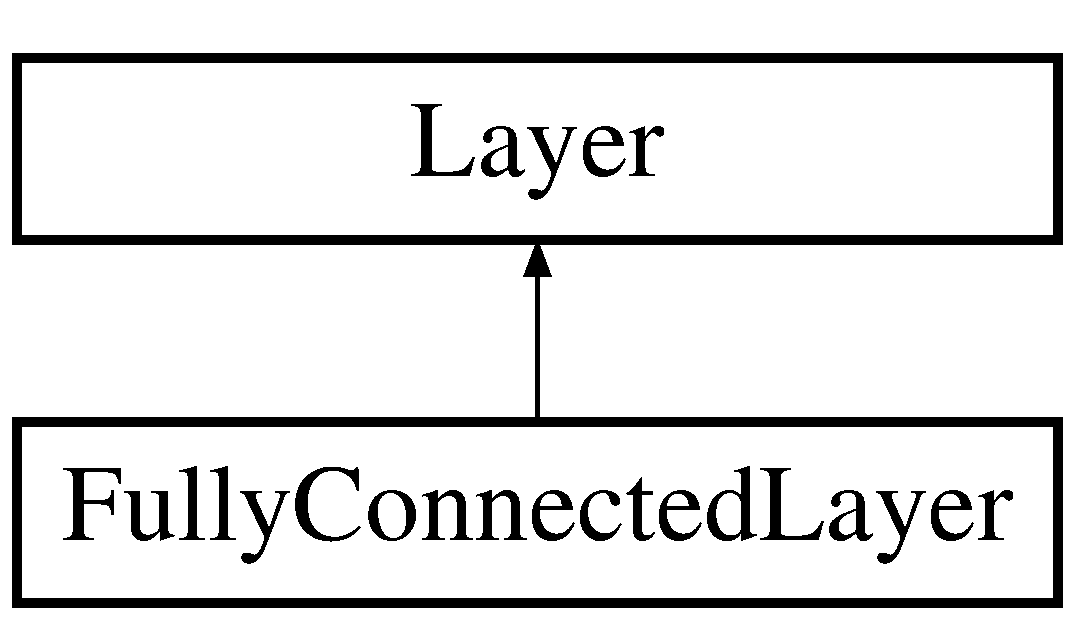
\includegraphics[height=2.000000cm]{class_fully_connected_layer}
\end{center}
\end{figure}
\subsection*{Public Member Functions}
\begin{DoxyCompactItemize}
\item 
\hypertarget{class_fully_connected_layer_a4bceb4e39fe4e7a716ce50210de3a988}{{\bfseries Fully\+Connected\+Layer} (int \+\_\+fanin, int \+\_\+fanout)}\label{class_fully_connected_layer_a4bceb4e39fe4e7a716ce50210de3a988}

\item 
\hypertarget{class_fully_connected_layer_a76e1fc371040de4e52cbe23c99901840}{{\bfseries Fully\+Connected\+Layer} (const \hyperlink{struct_config}{Config} \&cfg)}\label{class_fully_connected_layer_a76e1fc371040de4e52cbe23c99901840}

\item 
\hypertarget{class_fully_connected_layer_adba270546f0865b3adfb2739fcd7818e}{void {\bfseries Setup} (int \+\_\+stride, int \+\_\+side, int \+\_\+fanin, int \+\_\+fanout)}\label{class_fully_connected_layer_adba270546f0865b3adfb2739fcd7818e}

\item 
\hypertarget{class_fully_connected_layer_a13326e661fb3459d05653972d8ed0e5c}{void {\bfseries Set\+Weight} (const Mat\+Type \&)}\label{class_fully_connected_layer_a13326e661fb3459d05653972d8ed0e5c}

\item 
\hypertarget{class_fully_connected_layer_abc76d6caa38d466a2b58d824e50a9eb2}{void {\bfseries Set\+Input} (Mat\+Type $\ast$)}\label{class_fully_connected_layer_abc76d6caa38d466a2b58d824e50a9eb2}

\item 
\hypertarget{class_fully_connected_layer_a71b13c03aed1aa3b97920279e3534f7b}{void {\bfseries Apply\+Filter} ()}\label{class_fully_connected_layer_a71b13c03aed1aa3b97920279e3534f7b}

\item 
\hypertarget{class_fully_connected_layer_aeaa164864cf41ae5fe116cf8533a1817}{void {\bfseries Apply\+Nonlinearity} ()}\label{class_fully_connected_layer_aeaa164864cf41ae5fe116cf8533a1817}

\item 
\hypertarget{class_fully_connected_layer_ae769cfe87e16198f8b0959f87bfb3100}{void {\bfseries Down\+Sample} ()}\label{class_fully_connected_layer_ae769cfe87e16198f8b0959f87bfb3100}

\end{DoxyCompactItemize}
\subsection*{Public Attributes}
\begin{DoxyCompactItemize}
\item 
\hypertarget{class_fully_connected_layer_a3cf0cc240abfd47b8ce17c0f9886612b}{Mat\+Type {\bfseries Weight}}\label{class_fully_connected_layer_a3cf0cc240abfd47b8ce17c0f9886612b}

\item 
\hypertarget{class_fully_connected_layer_aa06f43fdb5f8d9bd9ae2f4501d5eea72}{Mat\+Type $\ast$ {\bfseries indata}}\label{class_fully_connected_layer_aa06f43fdb5f8d9bd9ae2f4501d5eea72}

\item 
\hypertarget{class_fully_connected_layer_a9dc1c3ddd28ba88594438e9029493cee}{Mat\+Type \hyperlink{class_fully_connected_layer_a9dc1c3ddd28ba88594438e9029493cee}{outdata}}\label{class_fully_connected_layer_a9dc1c3ddd28ba88594438e9029493cee}

\begin{DoxyCompactList}\small\item\em The input data. \end{DoxyCompactList}\item 
\hypertarget{class_fully_connected_layer_aed6f8602d64c19b1086e99e00edf09d1}{int {\bfseries fanin}}\label{class_fully_connected_layer_aed6f8602d64c19b1086e99e00edf09d1}

\item 
\hypertarget{class_fully_connected_layer_a6f06e1152dedcc402cb69161293a818e}{int {\bfseries fanout}}\label{class_fully_connected_layer_a6f06e1152dedcc402cb69161293a818e}

\item 
\hypertarget{class_fully_connected_layer_a0f1df8475560dd0fd422f1da735f6993}{string {\bfseries name}}\label{class_fully_connected_layer_a0f1df8475560dd0fd422f1da735f6993}

\end{DoxyCompactItemize}


The documentation for this class was generated from the following files\+:\begin{DoxyCompactItemize}
\item 
/\+Users/chengtai/\+Documents/2014/\+M\+O\+T\+R/modules/\+Alpha/\+Alpha/\hyperlink{layer_8h}{layer.\+h}\item 
/\+Users/chengtai/\+Documents/2014/\+M\+O\+T\+R/modules/\+Alpha/\+Alpha/layer.\+cpp\end{DoxyCompactItemize}

\hypertarget{class_layer}{\section{Layer Class Reference}
\label{class_layer}\index{Layer@{Layer}}
}


{\ttfamily \#include $<$layer.\+h$>$}

Inheritance diagram for Layer\+:\begin{figure}[H]
\begin{center}
\leavevmode
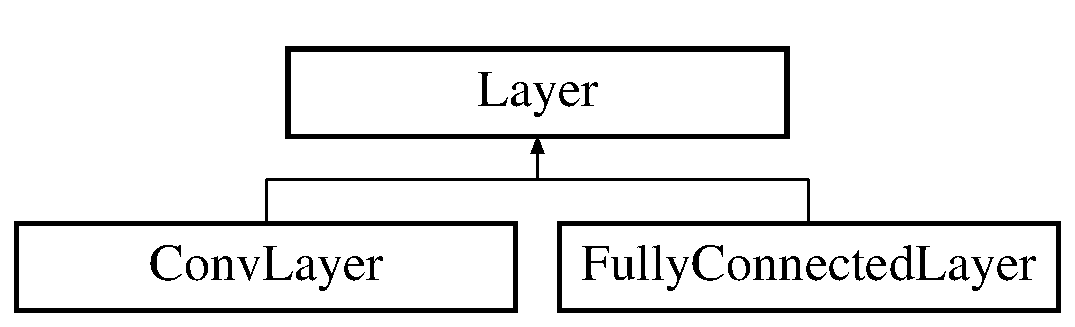
\includegraphics[height=2.000000cm]{class_layer}
\end{center}
\end{figure}
\subsection*{Public Member Functions}
\begin{DoxyCompactItemize}
\item 
\hyperlink{class_layer_a8f623c7c4737dc29ecc86978d243ac6f}{Layer} ()
\item 
virtual \hyperlink{class_layer_a2bac093f2a650095a5551fc455d10dc5}{$\sim$\+Layer} ()
\item 
virtual void \hyperlink{class_layer_acb52658f0eb1ec6f693dae392667d699}{Apply\+Filter} ()
\item 
virtual void \hyperlink{class_layer_aa351b47cff9c43788aabfd32bfc54176}{Downsample} ()
\item 
virtual void \hyperlink{class_layer_aab2270f2a6793112a8fa5aefe33eed1e}{Apply\+Nonlinearity} ()
\end{DoxyCompactItemize}
\subsection*{Public Attributes}
\begin{DoxyCompactItemize}
\item 
string \hyperlink{class_layer_ad7b365801548fd195fb0e1d48627f2f6}{name}
\end{DoxyCompactItemize}


\subsection{Detailed Description}


Definition at line 18 of file layer.\+h.



\subsection{Constructor \& Destructor Documentation}
\hypertarget{class_layer_a8f623c7c4737dc29ecc86978d243ac6f}{\index{Layer@{Layer}!Layer@{Layer}}
\index{Layer@{Layer}!Layer@{Layer}}
\subsubsection[{Layer}]{\setlength{\rightskip}{0pt plus 5cm}Layer\+::\+Layer (
\begin{DoxyParamCaption}
{}
\end{DoxyParamCaption}
)\hspace{0.3cm}{\ttfamily [inline]}}}\label{class_layer_a8f623c7c4737dc29ecc86978d243ac6f}


Definition at line 20 of file layer.\+h.

\hypertarget{class_layer_a2bac093f2a650095a5551fc455d10dc5}{\index{Layer@{Layer}!````~Layer@{$\sim$\+Layer}}
\index{````~Layer@{$\sim$\+Layer}!Layer@{Layer}}
\subsubsection[{$\sim$\+Layer}]{\setlength{\rightskip}{0pt plus 5cm}virtual Layer\+::$\sim$\+Layer (
\begin{DoxyParamCaption}
{}
\end{DoxyParamCaption}
)\hspace{0.3cm}{\ttfamily [virtual]}}}\label{class_layer_a2bac093f2a650095a5551fc455d10dc5}


\subsection{Member Function Documentation}
\hypertarget{class_layer_acb52658f0eb1ec6f693dae392667d699}{\index{Layer@{Layer}!Apply\+Filter@{Apply\+Filter}}
\index{Apply\+Filter@{Apply\+Filter}!Layer@{Layer}}
\subsubsection[{Apply\+Filter}]{\setlength{\rightskip}{0pt plus 5cm}virtual void Layer\+::\+Apply\+Filter (
\begin{DoxyParamCaption}
{}
\end{DoxyParamCaption}
)\hspace{0.3cm}{\ttfamily [virtual]}}}\label{class_layer_acb52658f0eb1ec6f693dae392667d699}


Reimplemented in \hyperlink{class_fully_connected_layer_a71b13c03aed1aa3b97920279e3534f7b}{Fully\+Connected\+Layer}, and \hyperlink{class_conv_layer_a70111098046a07416fcbdffdbe8f0cfd}{Conv\+Layer}.

\hypertarget{class_layer_aab2270f2a6793112a8fa5aefe33eed1e}{\index{Layer@{Layer}!Apply\+Nonlinearity@{Apply\+Nonlinearity}}
\index{Apply\+Nonlinearity@{Apply\+Nonlinearity}!Layer@{Layer}}
\subsubsection[{Apply\+Nonlinearity}]{\setlength{\rightskip}{0pt plus 5cm}virtual void Layer\+::\+Apply\+Nonlinearity (
\begin{DoxyParamCaption}
{}
\end{DoxyParamCaption}
)\hspace{0.3cm}{\ttfamily [virtual]}}}\label{class_layer_aab2270f2a6793112a8fa5aefe33eed1e}


Reimplemented in \hyperlink{class_fully_connected_layer_aeaa164864cf41ae5fe116cf8533a1817}{Fully\+Connected\+Layer}, and \hyperlink{class_conv_layer_a5e5a5da58cb21ca2894ecf55088a2636}{Conv\+Layer}.

\hypertarget{class_layer_aa351b47cff9c43788aabfd32bfc54176}{\index{Layer@{Layer}!Downsample@{Downsample}}
\index{Downsample@{Downsample}!Layer@{Layer}}
\subsubsection[{Downsample}]{\setlength{\rightskip}{0pt plus 5cm}virtual void Layer\+::\+Downsample (
\begin{DoxyParamCaption}
{}
\end{DoxyParamCaption}
)\hspace{0.3cm}{\ttfamily [virtual]}}}\label{class_layer_aa351b47cff9c43788aabfd32bfc54176}


\subsection{Member Data Documentation}
\hypertarget{class_layer_ad7b365801548fd195fb0e1d48627f2f6}{\index{Layer@{Layer}!name@{name}}
\index{name@{name}!Layer@{Layer}}
\subsubsection[{name}]{\setlength{\rightskip}{0pt plus 5cm}string Layer\+::name}}\label{class_layer_ad7b365801548fd195fb0e1d48627f2f6}


Definition at line 25 of file layer.\+h.



The documentation for this class was generated from the following file\+:\begin{DoxyCompactItemize}
\item 
\hyperlink{layer_8h}{layer.\+h}\end{DoxyCompactItemize}

\chapter{File Documentation}
\hypertarget{layer_8h}{\section{/\+Users/chengtai/\+Documents/2014/\+M\+O\+T\+R/modules/\+Alpha/\+Alpha/layer.h File Reference}
\label{layer_8h}\index{/\+Users/chengtai/\+Documents/2014/\+M\+O\+T\+R/modules/\+Alpha/\+Alpha/layer.\+h@{/\+Users/chengtai/\+Documents/2014/\+M\+O\+T\+R/modules/\+Alpha/\+Alpha/layer.\+h}}
}
{\ttfamily \#include \char`\"{}utils.\+h\char`\"{}}\\*
{\ttfamily \#include \char`\"{}helper.\+h\char`\"{}}\\*
{\ttfamily \#include \char`\"{}configuration.\+h\char`\"{}}\\*
\subsection*{Classes}
\begin{DoxyCompactItemize}
\item 
class \hyperlink{class_layer}{Layer}
\item 
class \hyperlink{class_conv_layer}{Conv\+Layer}
\item 
class \hyperlink{class_fully_connected_layer}{Fully\+Connected\+Layer}
\end{DoxyCompactItemize}


\subsection{Detailed Description}
This is the definition for convolutional layers and fully connected layers.


\begin{DoxyParams}{Parameters}
{\em \+\_\+ninmaps} & Number of input maps. \\
\hline
{\em \+\_\+inputrows} & Number of rows of input matrix. \\
\hline
{\em \+\_\+inputcols} & Number of columns of input matrix. \\
\hline
{\em \+\_\+noutmaps} & Number of maps of this layer. \\
\hline
{\em \+\_\+stride} & stride. \\
\hline
{\em \+\_\+side} & side. \\
\hline
{\em \+\_\+kernelsize} & kernelsize, must be square. \\
\hline
{\em \+\_\+indata.} & Input data, optional. \\
\hline
\end{DoxyParams}

%--- End generated contents ---

% Index
\newpage
\phantomsection
\addcontentsline{toc}{chapter}{Index}
\printindex

\end{document}
